%=========================================================================

\chapter{Introduction}
\todo[inline]{Klasicky popis toho co se tady bude dit, jak je to dulezite, atd.}

\chapter{Neural networks} 
General idea of neural networks was slowly emerging after World War II. Perceptron, as a single neuron unit, was created in 1958 by Frank Rosenblatt\footnote{The perceptron: A probabilistic model for information storage and organization in the brain. Rosenblatt, F. Psychological Review, Vol 65(6), Nov 1958, 386--408.}, but became popular only after creation of backpropagation algorithm in 1975. At that time neural nets have not reached massive popularity, not because they are not working, but due to small computing power of machines back then and lack of datasets. Recently (after 2000) neural nets became popular again, rebranded as \textquoteleft Deep Learning\textquoteright, because researchers realized that it is possible and very useful to stack neural nets on top of each other and create deep architectures, which are more practical than shallow ones. During this reinvention neural nets have been successfully applied in multiple fields like computer vision, speech recognition and natural language processing.

Since then various useful architectures and algorithms are now introduced almost every month. There is vast amount of various architectures and algorithms, in this chapter, I will describe only a couple -- those used in this thesis.

	\section{Recurrent neural nets}
Feedforward neural nets are extremely powerful models, which can be highly parallelized. Despite that, they can be only applied to problems with inputs and outputs, which have fixed dimensionality (e.g. one-hot encoding vectors). This is a serious drawback, as many of the real-world problems are defined as sequences with lengths that are unknown to us in beforehand. Soon recurrent neural networks were introduced and they proved to be very useful to this kind of task. There is vast amount of recurrent neural networks, many not suitable for sequential tasks like Hopfield network, which are very successful in specific tasks, but nevertheless not useful for us now.

Apart from classification, which can be more precise when using sequences, one of the most important tasks is next value prediction. This core task can be then extended very simply to predict arbitrary number of future values. Prediction problems are all around us, from the weather forecast and stock market prediction to the autocomplete in smartphones or web browsers.

\begin{figure}[!ht]
	\centering
	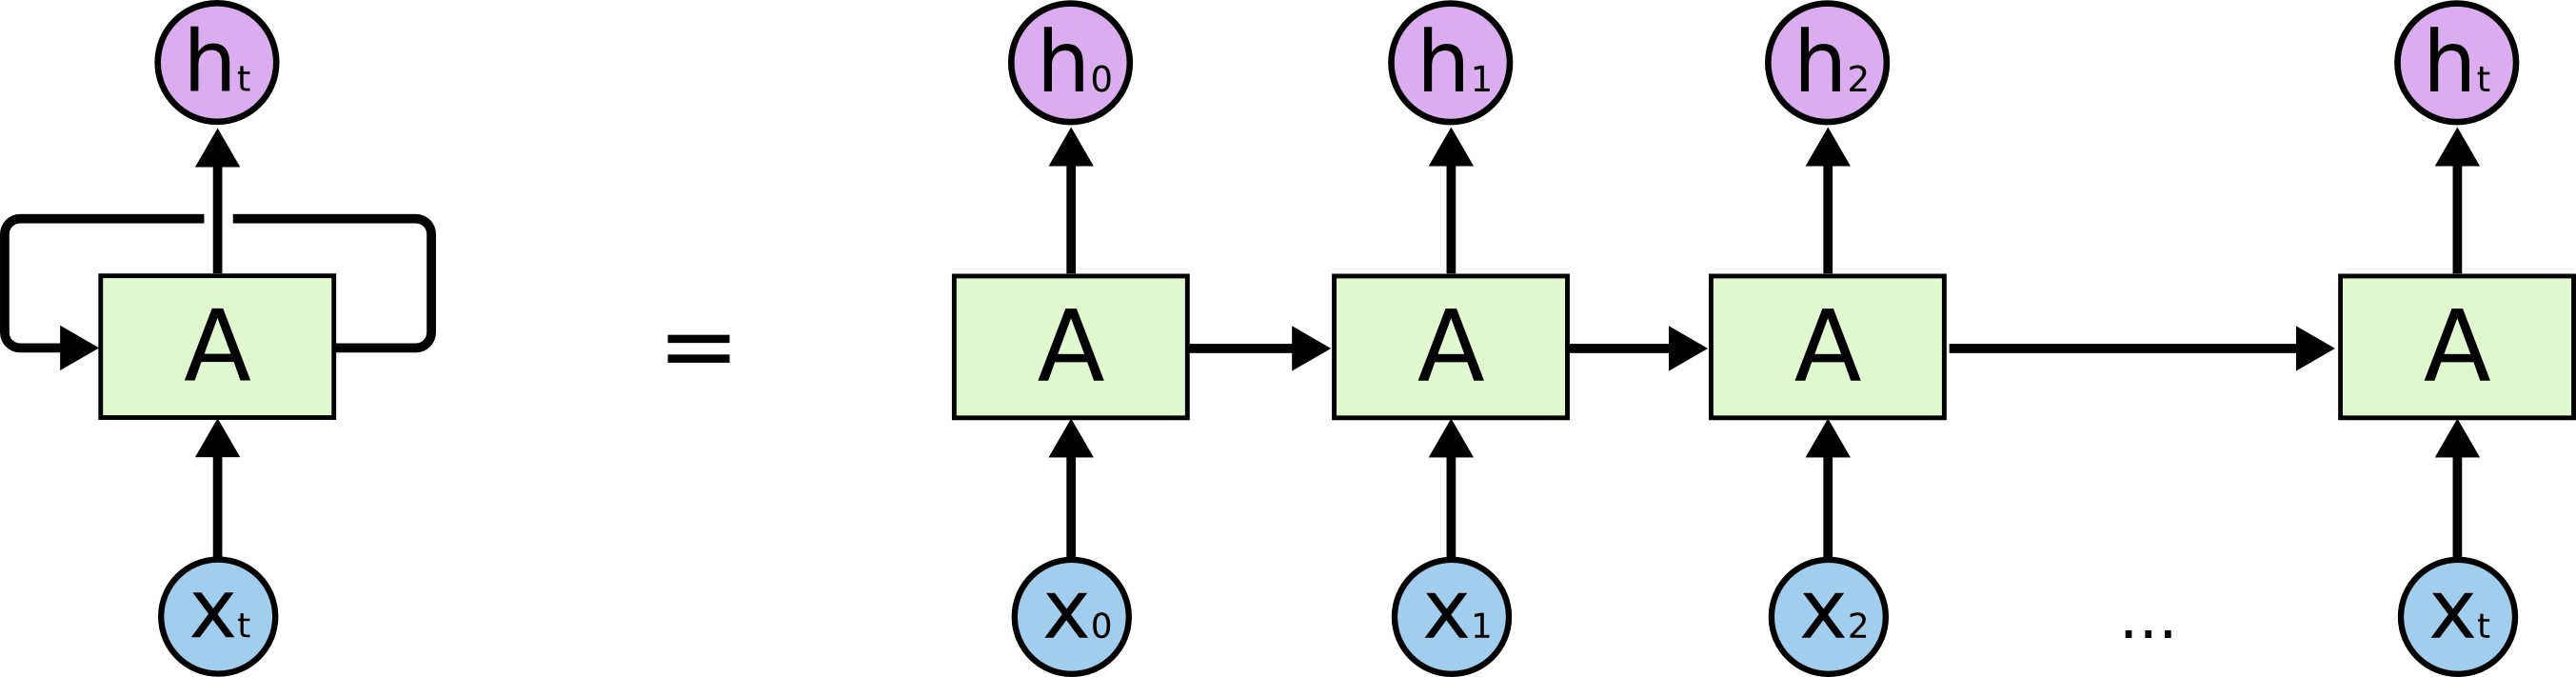
\includegraphics[width=0.7\textwidth]{fig/RNN-unrolled.png}
	\caption{Unrolling of the recurrent neural net. (C. Olah 2015)
		\label{fig:rnn-unroll}}
\end{figure}
%reference http://colah.github.io/posts/2015-08-Understanding-LSTMs/

We can understand recurrent neural networks as very deep forward nets with shared weights. It is called RNN unrolling and it is described in figure \ref{fig:rnn-unroll}. Layers of this very deep net spread in time, together with the input sequence. This is very innovative idea, which enabled training RNN with backpropagation through time. It also shows that, as very deep networks, they have vanishing or exploding gradient problem, which means that the network is not able to learn long-term dependencies, even though in theory it should. This is a serious issue, \todof{Mam to tady rozebrat vice?} which is caused by iterating many times over the weights and the activation function with derivatives $>1$ (exploding gradient) or $<1$ (vanishing gradient). Gradient then dies out and learning stops for distant dependencies. Among others this problem has been solved by the LSTM unit described in part \ref{subsec:lstm}, which is most popular now and following research resulting in GRU described in part \ref{subsec:gru}.

		\subsection{LSTM -- Long Short-Term Memory}\label{subsec:lstm}

Long Short-Term Memory nets are special kind of recurrent network, capable of learning long-term dependencies. This architecture was introduced by Hochreiter \& Schmidhuber (1997) in \cite{Hochreiter:1997:LSM:1246443.1246450} after prior research of vanishing gradient problem. Later architecture was refined and popularized by other researchers and nowadays LSTM is most used and popular RNN architecture used.

The LSTM unit designed that it can remember a value for an arbitrary length of time. It contains gates that determine when the input is significant enough to remember, when it should continue to remember or forget the value, and when it should output the value. All these gates are built from simple layers and mathematical operations, and have the same input - current network input, last output of the unit and hidden state value of the unit. Diagram of an LSTM unit is on the figure \ref{fig:lstm-unroll}.

\begin{figure}[!ht]
	\centering
	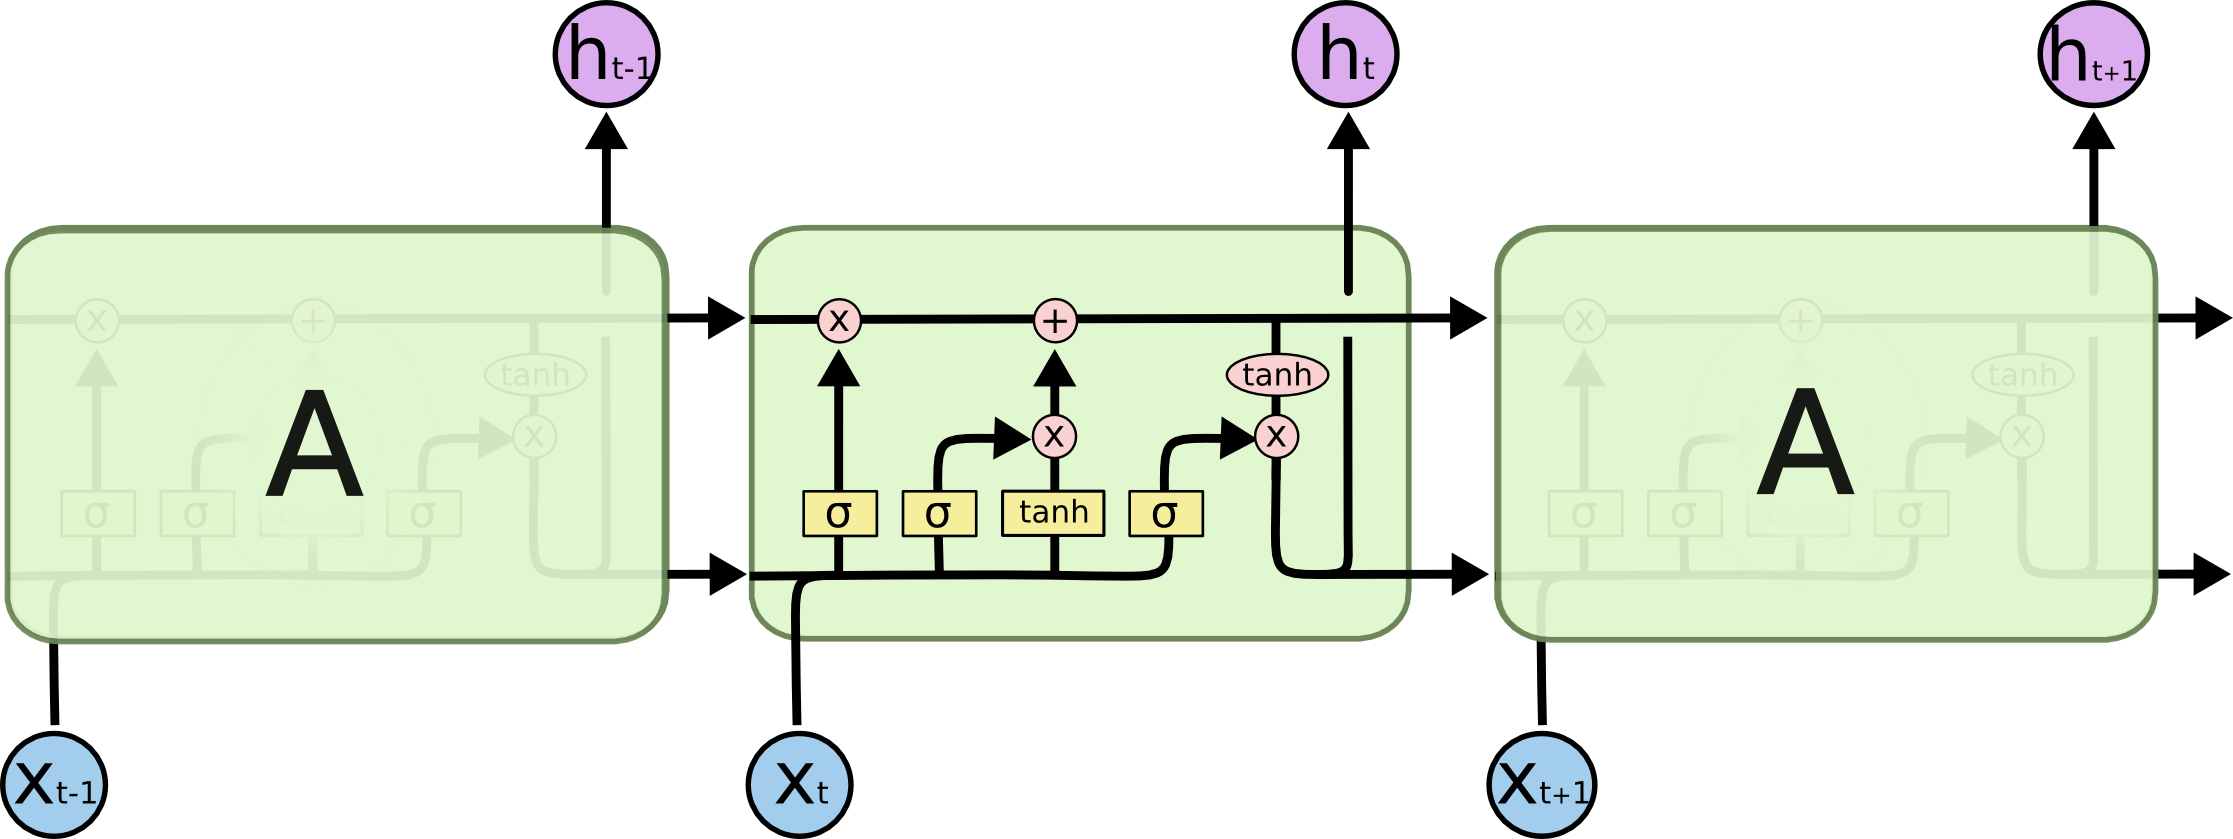
\includegraphics[width=0.9\textwidth]{./fig/LSTM3-chain.png}
	\caption{Unrolled LSTM unit. (C. Olah 2015)
		\label{fig:lstm-unroll}}
\end{figure}
%reference http://colah.github.io/posts/2015-08-Understanding-LSTMs/

\todo[inline]{Jak to vyresilo problem vyse. Pridat i rovnice, ktere pouzivam ja, rozebrat dopodrobna.}

\begin{figure}[!ht]
	\centering
	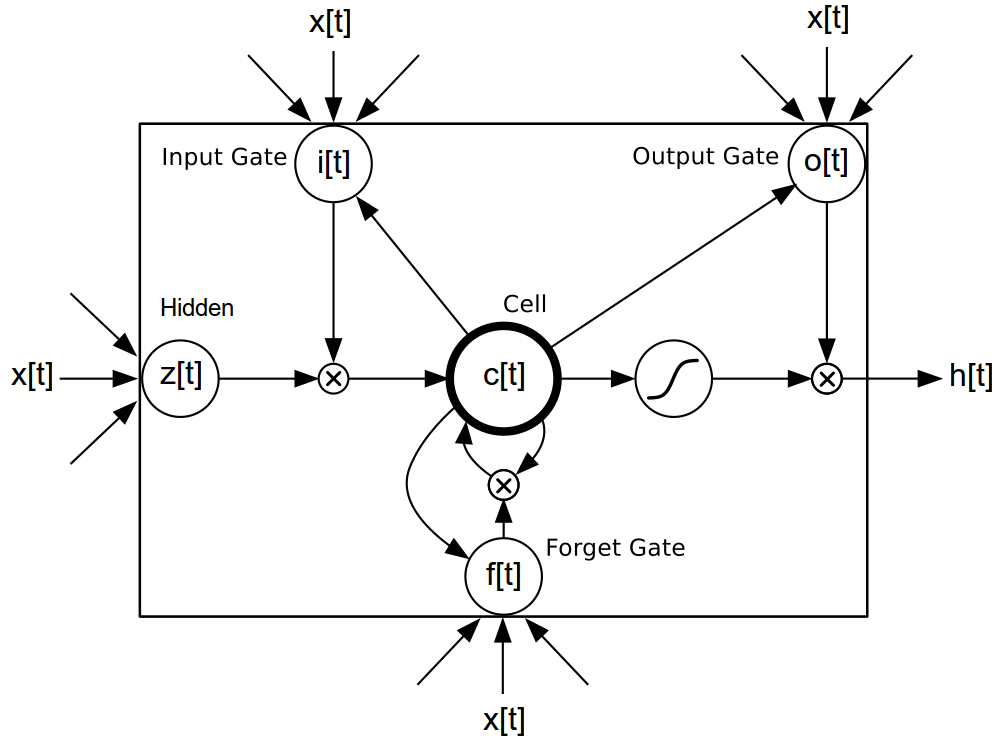
\includegraphics[width=0.7\textwidth]{./fig/LSTM-equations.png}
	\caption{LSTM unit for equations
		\label{fig:lstm-equations}}
\end{figure}

\begin{align}
	i_t &= \sigma(W_x^ix_t + W_h^ih_{t-1} + W_c^ic_{t-1} + b^i) \label{eq:lstm1}\\
	f_t &= \sigma(W_x^fx_t + W_h^fh_{t-1} + W_c^fc_{t-1} + b^f) \label{eq:lstm2}
\end{align}

\eqref{eq:lstm1}

\ref{eq:lstm2}

		\subsection{GRU -- Gated Recurrent Unit}\label{subsec:gru}
\todo[inline]{Zminit jako updatovanou verzi}
\cite{DBLP:journals/corr/ChoMGBSB14}
\cite{DBLP:journals/corr/GreffSKSS15}

		\subsection{Text sequences -- Word level embeddings and character level}
\todo[inline]{Mozna trochu upravit nazev. (Character level and word level embeddings)}
\todo[inline]{Popis toho jak se pracuje s textem v rnn, ze to je taky sekvence. Character level, word level, embeddings. Popis rozdilu toho jak funguji preklady a generovani dalsiho prvku sekvence.}

	\section{Convolutional neural nets}
\todo[inline]{Kratky uvod do toho, kde se pouzivaji, jak se vyvinuly, jednoduchy popis toho jak funguji. Obrazek?}
\todo[inline]{Asi neni potreba davat subsekce na vrstvy, staci popsat jak to funguje vsechno dohromady, jednotlive vrstvy ve vetach v jednom odstavci. Obrazek. V diplomce rozpracovat vic.}

%		\subsection{Convolutional layer}
%
%		\subsection{Pooling layer}

\chapter{Experiments}
\todo[inline, color=magenta!60]{Kapitola jen na semestralni projekt. V diplomce ji odstranim.}
\todo[inline]{Jak se to implementuje, jake knihovny se pouzivaji - Caffe, Theano, TensorFlow, Torch. Popsat ze Torch bude v tehle kapitole.}
\todo[inline]{Budu popisovat veci co jsem zkousel implementovat v Torchi.}

	\section{Torch}
\todo[inline, color=cyan!60]{Torch se zrecykluje do diplomky.}
\todo[inline]{Udelat tady tabulku o ruznych balicich co torch ma}
\todo[inline]{Jak funguji rekurentni site v Torchi.}
\todo[inline]{Nacitani modelu z Caffe, ukladani v Torchi...}
\cite{TorchLib}

		\subsection{nn, nngraph}
		\todo[inline]{Linky na knihovny v poznamkach pod carou.}
		
		\subsection{rnn}
		
		\subsection{Other packages}
		\todo[inline]{loadcaffe, optim,...}

	\section{Predicting next character in sequence}
\todo[inline]{Jak jsem to udelal, co to dela, ukazky.}
\todo[inline]{Reference na Karpathyho char-rnn}
\cite{char-rnn}

\chapter{Image caption generation}
\todo[inline]{Znovu uvod k tomu jak je to dulezite a tentokrat jak na tom lidi pracuji, co je potreba a jak se to hodnoti.}

	\section{Related Work}
\todo[inline]{Dat tomu nejake lepsi jmeno, clanky o popisovani obrazku ktere jsem cetl, pouzil.}

		\subsection{Show and Tell}
		\cite{DBLP:journals/corr/VinyalsTBE14}
		\cite{DBLP:journals/corr/SutskeverVL14}
		
		\todo[inline]{Clanek z Coco od Googlu.}
		\todo[inline]{Zminit i strojovy preklad (Sequence to Sequence Learning with Neural Networks), architektura encoder, decoder}
		
		\subsection{Show, Attend and Tell}
		\cite{DBLP:journals/corr/XuBKCCSZB15}
		
		\todo[inline]{Clanek z Coco z Montrealu/Toronta}
		
		\subsection{From Captions to Visual Concepts and Back}
		\cite{DBLP:journals/corr/FangGISDDGHMPZZ14}
		
		\todo[inline]{Clanek z Coco od Microsoftu, mrknout se i na pokracovani v druhem clanku}
		
		\subsection{Long-term Recurrent Convolutional Networks for Visual Recognition and Description}
		\cite{DBLP:journals/corr/DonahueHGRVSD14}
		\todo[inline]{Clanek z Coco z berkeley}


	\section{Datasets}
\todo[inline]{COCO, Flicker, popis jake jsou. Asi zrusit sekce, udelat jen tabulku a mensi popis.}
	
		\subsection{MS COCO}
		\cite{dataset-coco}
		
		\subsection{Flickr 30k,8k}
		\cite{dataset-flickr30k}
		\cite{dataset-flickr8k}
		
		\subsection{CIDEr datasets}
		\cite{Vedantam_2015_CVPR}		

	\section{Evaluation metrics}
\todo[inline]{BLEU, cIDER, jak se pouzivaji, co delaji...}
		\subsection{BLEU}
		\cite{Papineni:2002:BMA:1073083.1073135}
		
		\subsection{CIDEr}
		\cite{Vedantam_2015_CVPR}
		
		\subsection{METEOR}
		\cite{Lavie:2007:MAM:1626355.1626389}

\chapter{Model}
\todo[inline, color=cyan!60]{Do semestralniho projektu nebo az na diplomku?}
\todo[inline]{Design modelu, co chci pouzit, jake metody chci zkusit.}
\todo[inline]{Polozit si principialni otazku a zjistit jestli to nejak pomuze, jak to funguje.}

	\section{Architecture}
\todo[inline]{Architektura modelu, jake matematicke modely jsem pouzil, bez implementacnich detailu.}

	\section{Training details}
\todo[inline]{Popis pomoci jakeho algoritmu jsme trenovali, s jakyma parametrama, minibatches, datasety.}

%\chapter{Implementation}
%\todo[inline, color=cyan!60]{Bude az v diplomce, ne semestralnim projektu}
%
%	\section{Torch framework}
%\todo[inline]{Popis Torche, ruznych druhu modulu ktere ma, ktere jsem pouzil ja.}
%
%	\section{Parallelization}
%\todo[inline]{Nejaky popis toho ze to lze trenovat na gpu, jak se to dela v Torchi..}	
%
%\chapter{Results and model evaluation}
%\todo[inline, color=cyan!60]{Bude az v diplomce, ne semestralnim projektu}
%\todo[inline]{Performance, analysis,... spravne pojmenovat}
%\todo[inline]{Kde se trenovalo? Na jakych strojich? Jak to bylo rychle? Jak to bylo na cpu pomale?}
%
%	\section{Speed}
%\todo[inline]{Jak bylo trenovani rychle, }

\chapter{Conclusion}
\todo[inline]{Udelat jeden zaver pro semestralni projekt, pak ho prepsat pro diplomku.}
%=========================================================================
